\documentclass[nooutcomes]{ximera}

\graphicspath{
  {./}
  {1-1QuantitativeReasoning/}
  {1-2RelationsAndGraphs/}
  {1-3ChangingInTandem/}
  {2-1LinearEquations/}
  {2-2LinearModeling/}
  {2-3ExponentialModeling/}
  {3-1WhatIsAFunction/}
  {3-2FunctionProperties/}
  {3-3AverageRatesOfChange/}
  {4-1BuildingNewFunctions/}
  {4-2Quadratics/}
  {4-3Polynomials/}
  {4-4Roots/}
  {5-1IntroToTransformations/}
  {5-2ExponentialFunctions/}
  {5-3IntroToLogarithms/}
  {6-1RationalFunctions/}
  {6-2DomainandRangeRevisited/}
  {6-3AsympOfRationalFunctions/}
  {7-0Review/}
  {7-1CompositionOfFunctions/}
  {7-2ZerosOfFunctions/}
  {7-3FunctionTransformationsRevisited/}
  {7-4SolvingInequalities/}
  {8-1FunctionTransformations/}
  {8-2SolvingInequalities/}
  {7-5FunctionTransformationsProject/}
  {8-1RightTriangleTrig/}
  {8-2TheUnitCircle/}
  {8-3TrigIdentities/}
  {9-1UnitCircleToFunctionGraph/}
  {9-2TrigFunctions/}
  {9-3TrigTransformations/}
  {9-4SomeApplicationsOfTrig/}
  {10-1InverseFunctionsRevisited/}
  {10-2Logarithms/}
  {10-3InverseTrig/}
  {11-1SystemsOfEquations/}
  {11-2NonlinearSystems/}
  {11-3ApplicationsOfSystems/}
  {11-4SecantLinesRevisited/}
  {11-5FunctionsTheBigPicture/}
  {14-1DisplacementVsDistance/}
  {1-1QuantitativeReasoning/exercises/}
  {1-2RelationsAndGraphs/exercises/}
  {../1-3ChangingInTandem/exercises/}
  {../2-1LinearEquations/exercises/}
  {../2-2LinearModeling/exercises/}
  {../2-3ExponentialModeling/exercises/}
  {../3-1WhatIsAFunction/exercises/}
  {../3-2FunctionProperties/exercises/}
  {../3-3AverageRatesOfChange/exercises/}
  {../5-2ExponentialFunctions/exercises/}
  {../4-1BuildingNewFunctions/exercises/}
  {../4-2Quadratics/exercises/}
 {../4-3Polynomials/exercises/}
 {../4-4Roots/exercises/}
  {../5-1RationalFunctions/exercises/}
  {../6-1Domain/exercises/}
  {../6-2Range/exercises/}
  {../6-3CompositionOfFunctions/exercises/}
  {../7-1ZerosOfFunctions/exercises/}
  {../7-XZerosOfPolynomials/exercises/}
  {../7-2ZerosOfFamousFunctions/exercises/}
  {../8-1FunctionTransformations/exercises/}
  {../11-1SystemsOfEquations/exercises/}
  {../7-5FunctionTransformationsProject/exercises/}
  {../7-0Review/exercises/}
  {../7-4SolvingInequalities/exercises/}
  {../7-5FunctionTransformationsProject/exercises/}
  {../8-1RightTriangleTrig/exercises/}
  {../8-2TheUnitCircle/exercises/}
  {../8-3TrigIdentities/exercises/}
  {../9-1UnitCircleToFunctionGraph/exercises/}
  {../9-2TrigFunctions/exercises/}
  {../9-3TrigTransformations/exercises/}
  {../9-4SomeApplicationsOfTrig/exercises/}
  {../10-1InverseFunctionsRevisited/exercises/}
  {../10-2Logarithms/exercises/}
  {../10-3InverseTrig/exercises/}
  {../11-1SystemsOfEquations/exercises/}
  {../11-2NonlinearSystems/exercises/}
  {../11-3ApplicationsOfSystems/exercises/}
  {../11-4SecantLinesRevisited/exercises/}
  {../11-5FunctionsTheBigPicture/exercises/}
  {../14-1DisplacementVsDistance/exercises/}
  {../5-1IntroToTransformations/exercises/}
  {../5-2ExponentialFunctions/exercises/}
  {../5-3IntroToLogarithms/exercises/}
  {../6-1RationalFunctions/exercises/}
  {../6-2DomainandRangeRevisited/exercises/}
  {../6-3AsympOfRationalFunctions/exercises/}
  {../7-1CompositionOfFunctions/exercises/}
  {../7-2ZerosOfFunctions/exercises/}
  {../7-3ZerosOfPolynomials/exercises/}
  {../7-4ZerosOfFamousFunctions/exercises/}
  {7-3FunctionTransformationsRevisited/exercises/}
  {7-4SolvingInequalities/exercises/}
}


%%%%%%%%%%%%%%%%%%%%%%%%%%%%%%%%%%%%%%%%%%%%%%%%%
\renewcommand{\link}[2][]{\href{#2}{\underline{#1}}% the optional argument,
                                       % a name for the link as a clickable link
\ifthenelse{\equal{#1}{}}% if no optional argument, then 
{\url{#2}}% just print the name
{
%\footnote{See #1 at \url{#2}}
}}% include the link address as a footnote
%%%%%%%%%%%%%%%%%%%%%%%%%%%%%%%%%%%%%%%%%%%%%%%%%%



\DeclareGraphicsExtensions{.pdf,.png,.jpg,.eps}

\newcommand{\mooculus}{\textsf{\textbf{MOOC}\textnormal{\textsf{ULUS}}}}

\newcommand{\av}{\mathrm{AROC}}

\newcommand{\tech}{Desmos}

\newcommand{\calcHW}{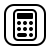
\includegraphics[width=0.5cm, trim={0 4mm 0 0}]{calc.png} \, }

\usepackage[makeroom]{cancel} %% for strike outs

\ifxake
\else
\usepackage[most]{tcolorbox}
\fi


%\typeout{************************************************}
%\typeout{New Environments}
%\typeout{************************************************}

%% to fix for web can be removed when deployed offically with ximera2
\let\image\relax\let\endimage\relax
\NewEnviron{image}{% 
  \begin{center}\BODY\end{center}% center
}



\NewEnviron{folder}{
      \addcontentsline{toc}{section}{\textbf{\BODY}}
}

%\ifxake
%\let\summary\relax
%\let\endsummary\relax
%\newtheorem*{summary}{Summary}
\newenvironment{callout}{\begin{remark}}{\end{remark}}
\newenvironment{overview}{\begin{remark}\textbf{Overview}~}{\end{remark}}
\newenvironment{objectives}{\begin{remark}\textbf{Objectives}\\}{\end{remark}}
\newenvironment{motivatingQuestions}{\begin{remark}\textbf{Motivating Questions}~}{\end{remark}}
\newenvironment{MM}{\begin{remark}\textbf{Metacognitive Moment}~}{\end{remark}}

      
%% NEEDED FOR XIMERA 2
%\ximerizedEnvironment{summary}
%\ximerizedEnvironment{callout}
%\ximerizedEnvironment{overview} 
%\ximerizedEnvironment{objectives}
%\ximerizedEnvironment{motivatingQuestions}
%\ximerizedEnvironment{MM}
%% \else
%% %% CALLOUT
%% \NewEnviron{callout}{
%%   \begin{tcolorbox}[colback=blue!5, breakable,pad at break*=1mm]
%%       \BODY
%%   \end{tcolorbox}
%% }
%% %% MOTIVATING QUESTIONS
%% \NewEnviron{motivatingQuestions}{
%%   \begin{tcolorbox}[ breakable,pad at break*=1mm]
%%     \textbf{\Large Motivating Questions}\hfill
%%     %\begin{itemize}[label=\textbullet]
%%       \BODY
%%     %\end{itemize}
%%   \end{tcolorbox}
%% }
%% %% OBJECTIVES
%% \NewEnviron{objectives}{  
%%     \vspace{.5in}
%%       %\begin{tcolorbox}[colback=orange!5, breakable,pad at break*=1mm]
%%     \textbf{\Large Learning Objectives}
%%     \begin{itemize}[label=\textbullet]
%%       \BODY
%%     \end{itemize}
%%     %\end{tcolorbox}
%% }
%% %% DEFINITION
%% \let\definition\relax
%% \let\enddefinition\relax
%% \NewEnviron{definition}{
%%   \begin{tcolorbox}[ breakable,pad at break*=1mm]
%%     \noindent\textbf{Definition}~
%%       \BODY
%%   \end{tcolorbox}
%% }
%% %% OVERVIEW
%% \let\overview\relax
%% \let\overview\relax
%% \NewEnviron{overview}{
%%   \begin{tcolorbox}[ breakable,pad at break*=1mm]
%%     \textbf{\Large Overview}
%%     %\begin{itemize}[label=\textbullet] %% breaks Xake
%%       \BODY
%%     %\end{itemize}
%%   \end{tcolorbox}
%% }
%% %% SUMMARY
%% \let\summary\relax
%% \let\endsummary\relax
%% \NewEnviron{summary}{
%%   \begin{tcolorbox}[ breakable,pad at break*=1mm]
%%     \textbf{\Large Summary}
%%     %\begin{itemize}[label=\textbullet] %% breaks Xake
%%       \BODY
%%     %\end{itemize}
%%   \end{tcolorbox}
%% }
%% %% REMARK
%% \let\remark\relax
%% \let\endremark\relax
%% \NewEnviron{remark}{
%%   \begin{tcolorbox}[colback=green!5, breakable,pad at break*=1mm]
%%     \noindent\textbf{Remark}~
%%       \BODY
%%   \end{tcolorbox}
%% }
%% %% EXPLANATION
%% \let\explanation\relax
%% \let\endexplanation\relax
%% \NewEnviron{explanation}{
%%     \normalfont
%%     \noindent\textbf{Explanation}~
%%       \BODY
%% }
%% %% EXPLORATION
%% \let\exploration\relax
%% \let\endexploration\relax
%% \NewEnviron{exploration}{
%%   \begin{tcolorbox}[colback=yellow!10, breakable,pad at break*=1mm]
%%     \noindent\textbf{Exploration}~
%%       \BODY
%%   \end{tcolorbox}
%% }
%% %% METACOGNITIVE MOMENTS
%% \let\MM\relax
%% \let\endMM\relax
%% \NewEnviron{MM}{
%%   \begin{tcolorbox}[colback=pink!15, breakable,pad at break*=1mm]
%%     \noindent\textbf{Metacognitive Moment}~
%%       \BODY
%%   \end{tcolorbox}
%% }


%% \fi





%Notes on what envirnoment to use:  Example with Explanation in text; if they are supposed to answer- Problem; no answer - Exploration


%\typeout{************************************************}
%% Header and footers
%\typeout{************************************************}

\newcommand{\licenseAcknowledgement}{Licensed under Creative Commons 4.0}
\newcommand{\licenseAPC}{\renewcommand{\licenseAcknowledgement}{\textbf{Acknowledgements:} Active Prelude to Calculus (https://activecalculus.org/prelude) }}
\newcommand{\licenseSZ}{\renewcommand{\licenseAcknowledgement}{\textbf{Acknowledgements:} Stitz Zeager Open Source Mathematics (https://www.stitz-zeager.com/) }}
\newcommand{\licenseAPCSZ}{\renewcommand{\licenseAcknowledgement}{\textbf{Acknowledgements:} Active Prelude to Calculus (https://activecalculus.org/prelude) and Stitz Zeager Open Source Mathematics (https://www.stitz-zeager.com/) }}
\newcommand{\licenseORCCA}{\renewcommand{\licenseAcknowledgement}{\textbf{Acknowledgements:} Original source material, products with readable and accessible
math content, and other information freely available at pcc.edu/orcca.}}
\newcommand{\licenseY}{\renewcommand{\licenseAcknowledgement}{\textbf{Acknowledgements:} Yoshiwara Books (https://yoshiwarabooks.org/)}}
\newcommand{\licenseOS}{\renewcommand{\licenseAcknowledgement}{\textbf{Acknowledgements:} OpenStax College Algebra (https://openstax.org/details/books/college-algebra)}}
\newcommand{\licenseAPCSZCSCC}{\renewcommand{\licenseAcknowledgement}{\textbf{Acknowledgements:} Source material includes: Active Prelude to Calculus (https://activecalculus.org/prelude), Stitz Zeager Open Source Mathematics (https://www.stitz-zeager.com/), CSCC PreCalculus and Calculus texts (https://ximera.osu.edu/csccmathematics)}}
\newcommand{\licenseAPCSZORCCA}{\renewcommand{\licenseAcknowledgement}{\textbf{Acknowledgements:} Source material includes: Active Prelude to Calculus (https://activecalculus.org/prelude), Stitz Zeager Open Source Mathematics (https://www.stitz-zeager.com/), ORCCA: Original source material, products with readable and accessible math content, and other information freely available at pcc.edu/orcca.}}


\ifxake\else %% do nothing on the website
\usepackage{fancyhdr}
\pagestyle{fancy}
\fancyhf{}
\fancyhead[R]{\sectionmark}
\fancyfoot[L]{\thepage}
\fancyfoot[C]{\begin{minipage}{.8\textwidth}\tiny\licenseAcknowledgement\end{minipage}}
\renewcommand{\headrulewidth}{0pt}
\renewcommand{\footrulewidth}{0pt}
\fi

%%%%%%%%%%%%%%%%



%\typeout{************************************************}
%\typeout{Table of Contents}
%\typeout{************************************************}


%% Edit this to change the font style
\newcommand{\sectionHeadStyle}{\sffamily\bfseries}


\makeatletter

%% part uses arabic numerals
\renewcommand*\thepart{\arabic{part}}


\ifxake\else
\renewcommand\chapterstyle{%
  \def\maketitle{%
    \addtocounter{titlenumber}{1}%
    \pagestyle{fancy}
    \phantomsection
    \addcontentsline{toc}{section}{\textbf{\thepart.\thetitlenumber\hspace{1em}\@title}}%
                    {\flushleft\small\sectionHeadStyle\@pretitle\par\vspace{-1.5em}}%
                    {\flushleft\LARGE\sectionHeadStyle\thepart.\thetitlenumber\hspace{1em}\@title \par }%
                    {\setcounter{problem}{0}\setcounter{sectiontitlenumber}{0}}%
                    \par}}





\renewcommand\sectionstyle{%
  \def\maketitle{%
    \addtocounter{sectiontitlenumber}{1}
    \pagestyle{fancy}
    \phantomsection
    \addcontentsline{toc}{subsection}{\thepart.\thetitlenumber.\thesectiontitlenumber\hspace{1em}\@title}%
    {\flushleft\small\sectionHeadStyle\@pretitle\par\vspace{-1.5em}}%
    {\flushleft\Large\sectionHeadStyle\thepart.\thetitlenumber.\thesectiontitlenumber\hspace{1em}\@title \par}%
    %{\setcounter{subsectiontitlenumber}{0}}%
    \par}}



\renewcommand\section{\@startsection{paragraph}{10}{\z@}%
                                     {-3.25ex\@plus -1ex \@minus -.2ex}%
                                     {1.5ex \@plus .2ex}%
                                     {\normalfont\large\sectionHeadStyle}}
\renewcommand\subsection{\@startsection{subparagraph}{10}{\z@}%
                                    {3.25ex \@plus1ex \@minus.2ex}%
                                    {-1em}%
                                    {\normalfont\normalsize\sectionHeadStyle}}

\fi

%% redefine Part
\renewcommand\part{%
   {\setcounter{titlenumber}{0}}
  \if@openright
    \cleardoublepage
  \else
    \clearpage
  \fi
  \thispagestyle{plain}%
  \if@twocolumn
    \onecolumn
    \@tempswatrue
  \else
    \@tempswafalse
  \fi
  \null\vfil
  \secdef\@part\@spart}

\def\@part[#1]#2{%
    \ifnum \c@secnumdepth >-2\relax
      \refstepcounter{part}%
      \addcontentsline{toc}{part}{\thepart\hspace{1em}#1}%
    \else
      \addcontentsline{toc}{part}{#1}%
    \fi
    \markboth{}{}%
    {\centering
     \interlinepenalty \@M
     \normalfont
     \ifnum \c@secnumdepth >-2\relax
       \huge\sffamily\bfseries \partname\nobreakspace\thepart
       \par
       \vskip 20\p@
     \fi
     \Huge \bfseries #2\par}%
    \@endpart}
\def\@spart#1{%
    {\centering
     \interlinepenalty \@M
     \normalfont
     \Huge \bfseries #1\par}%
    \@endpart}
\def\@endpart{\vfil\newpage
              \if@twoside
               \if@openright
                \null
                \thispagestyle{empty}%
                \newpage
               \fi
              \fi
              \if@tempswa
                \twocolumn
                \fi}



\makeatother





%\typeout{************************************************}
%\typeout{Stuff from Ximera}
%\typeout{************************************************}



\usepackage{array}  %% This is for typesetting long division
\setlength{\extrarowheight}{+.1cm}
\newdimen\digitwidth
\settowidth\digitwidth{9}
\def\divrule#1#2{
\noalign{\moveright#1\digitwidth
\vbox{\hrule width#2\digitwidth}}}





\newcommand{\RR}{\mathbb R}
\newcommand{\R}{\mathbb R}
\newcommand{\N}{\mathbb N}
\newcommand{\Z}{\mathbb Z}

\newcommand{\sagemath}{\textsf{SageMath}}


\def\d{\,d}
%\renewcommand{\d}{\mathop{}\!d}
\newcommand{\dd}[2][]{\frac{\d #1}{\d #2}}
\newcommand{\pp}[2][]{\frac{\partial #1}{\partial #2}}
\renewcommand{\l}{\ell}
\newcommand{\ddx}{\frac{d}{\d x}}



%\newcommand{\unit}{\,\mathrm}
\newcommand{\unit}{\mathop{}\!\mathrm}
\newcommand{\eval}[1]{\bigg[ #1 \bigg]}
\newcommand{\seq}[1]{\left( #1 \right)}
\renewcommand{\epsilon}{\varepsilon}
\renewcommand{\phi}{\varphi}


\renewcommand{\iff}{\Leftrightarrow}

\DeclareMathOperator{\arccot}{arccot}
\DeclareMathOperator{\arcsec}{arcsec}
\DeclareMathOperator{\arccsc}{arccsc}
\DeclareMathOperator{\sign}{sign}


%\DeclareMathOperator{\divergence}{divergence}
%\DeclareMathOperator{\curl}[1]{\grad\cross #1}
\newcommand{\lto}{\mathop{\longrightarrow\,}\limits}

\renewcommand{\bar}{\overline}

\colorlet{textColor}{black}
\colorlet{background}{white}
\colorlet{penColor}{blue!50!black} % Color of a curve in a plot
\colorlet{penColor2}{red!50!black}% Color of a curve in a plot
\colorlet{penColor3}{red!50!blue} % Color of a curve in a plot
\colorlet{penColor4}{green!50!black} % Color of a curve in a plot
\colorlet{penColor5}{orange!80!black} % Color of a curve in a plot
\colorlet{penColor6}{yellow!70!black} % Color of a curve in a plot
\colorlet{fill1}{penColor!20} % Color of fill in a plot
\colorlet{fill2}{penColor2!20} % Color of fill in a plot
\colorlet{fillp}{fill1} % Color of positive area
\colorlet{filln}{penColor2!20} % Color of negative area
\colorlet{fill3}{penColor3!20} % Fill
\colorlet{fill4}{penColor4!20} % Fill
\colorlet{fill5}{penColor5!20} % Fill
\colorlet{gridColor}{gray!50} % Color of grid in a plot

\newcommand{\surfaceColor}{violet}
\newcommand{\surfaceColorTwo}{redyellow}
\newcommand{\sliceColor}{greenyellow}




\pgfmathdeclarefunction{gauss}{2}{% gives gaussian
  \pgfmathparse{1/(#2*sqrt(2*pi))*exp(-((x-#1)^2)/(2*#2^2))}%
}





%\typeout{************************************************}
%\typeout{ORCCA Preamble.Tex}
%\typeout{************************************************}


%% \usepackage{geometry}
%% \geometry{letterpaper,total={408pt,9.0in}}
%% Custom Page Layout Adjustments (use latex.geometry)
%% \usepackage{amsmath,amssymb}
%% \usepackage{pgfplots}
\usepackage{pifont}                                         %needed for symbols, s.a. airplane symbol
\usetikzlibrary{positioning,fit,backgrounds}                %needed for nested diagrams
\usetikzlibrary{calc,trees,positioning,arrows,fit,shapes}   %needed for set diagrams
\usetikzlibrary{decorations.text}                           %needed for text following a curve
\usetikzlibrary{arrows,arrows.meta}                         %needed for open/closed intervals
\usetikzlibrary{positioning,3d,shapes.geometric}            %needed for 3d number sets tower

%% NEEDED FOR XIMERA 1
%\usetkzobj{all}       %NO LONGER VALID
%%%%%%%%%%%%%%

\usepackage{tikz-3dplot}
\usepackage{tkz-euclide}                     %needed for triangle diagrams
\usepgfplotslibrary{fillbetween}                            %shade regions of a plot
\usetikzlibrary{shadows}                                    %function diagrams
\usetikzlibrary{positioning}                                %function diagrams
\usetikzlibrary{shapes}                                     %function diagrams
%%% global colors from https://www.pcc.edu/web-services/style-guide/basics/color/ %%%
\definecolor{ruby}{HTML}{9E0C0F}
\definecolor{turquoise}{HTML}{008099}
\definecolor{emerald}{HTML}{1c8464}
\definecolor{amber}{HTML}{c7502a}
\definecolor{amethyst}{HTML}{70485b}
\definecolor{sapphire}{HTML}{263c53}
\colorlet{firstcolor}{sapphire}
\colorlet{secondcolor}{turquoise}
\colorlet{thirdcolor}{emerald}
\colorlet{fourthcolor}{amber}
\colorlet{fifthcolor}{amethyst}
\colorlet{sixthcolor}{ruby}
\colorlet{highlightcolor}{green!50!black}
\colorlet{graphbackground}{white}
\colorlet{wood}{brown!60!white}
%%% curve, dot, and graph custom styles %%%
\pgfplotsset{firstcurve/.style      = {color=firstcolor,  mark=none, line width=1pt, {Kite}-{Kite}, solid}}
\pgfplotsset{secondcurve/.style     = {color=secondcolor, mark=none, line width=1pt, {Kite}-{Kite}, solid}}
\pgfplotsset{thirdcurve/.style      = {color=thirdcolor,  mark=none, line width=1pt, {Kite}-{Kite}, solid}}
\pgfplotsset{fourthcurve/.style     = {color=fourthcolor, mark=none, line width=1pt, {Kite}-{Kite}, solid}}
\pgfplotsset{fifthcurve/.style      = {color=fifthcolor,  mark=none, line width=1pt, {Kite}-{Kite}, solid}}
\pgfplotsset{highlightcurve/.style  = {color=highlightcolor,  mark=none, line width=5pt, -, opacity=0.3}}   % thick, opaque curve for highlighting
\pgfplotsset{asymptote/.style       = {color=gray, mark=none, line width=1pt, <->, dashed}}
\pgfplotsset{symmetryaxis/.style    = {color=gray, mark=none, line width=1pt, <->, dashed}}
\pgfplotsset{guideline/.style       = {color=gray, mark=none, line width=1pt, -}}
\tikzset{guideline/.style           = {color=gray, mark=none, line width=1pt, -}}
\pgfplotsset{altitude/.style        = {dashed, color=gray, thick, mark=none, -}}
\tikzset{altitude/.style            = {dashed, color=gray, thick, mark=none, -}}
\pgfplotsset{radius/.style          = {dashed, thick, mark=none, -}}
\tikzset{radius/.style              = {dashed, thick, mark=none, -}}
\pgfplotsset{rightangle/.style      = {color=gray, mark=none, -}}
\tikzset{rightangle/.style          = {color=gray, mark=none, -}}
\pgfplotsset{closedboundary/.style  = {color=black, mark=none, line width=1pt, {Kite}-{Kite},solid}}
\tikzset{closedboundary/.style      = {color=black, mark=none, line width=1pt, {Kite}-{Kite},solid}}
\pgfplotsset{openboundary/.style    = {color=black, mark=none, line width=1pt, {Kite}-{Kite},dashed}}
\tikzset{openboundary/.style        = {color=black, mark=none, line width=1pt, {Kite}-{Kite},dashed}}
\tikzset{verticallinetest/.style    = {color=gray, mark=none, line width=1pt, <->,dashed}}
\pgfplotsset{soliddot/.style        = {color=firstcolor,  mark=*, only marks}}
\pgfplotsset{hollowdot/.style       = {color=firstcolor,  mark=*, only marks, fill=graphbackground}}
\pgfplotsset{blankgraph/.style      = {xmin=-10, xmax=10,
                                        ymin=-10, ymax=10,
                                        axis line style={-, draw opacity=0 },
                                        axis lines=box,
                                        major tick length=0mm,
                                        xtick={-10,-9,...,10},
                                        ytick={-10,-9,...,10},
                                        grid=major,
                                        grid style={solid,gray!20},
                                        xticklabels={,,},
                                        yticklabels={,,},
                                        minor xtick=,
                                        minor ytick=,
                                        xlabel={},ylabel={},
                                        width=0.75\textwidth,
                                      }
            }
\pgfplotsset{numberline/.style      = {xmin=-10,xmax=10,
                                        minor xtick={-11,-10,...,11},
                                        xtick={-10,-5,...,10},
                                        every tick/.append style={thick},
                                        axis y line=none,
                                        y=15pt,
                                        axis lines=middle,
                                        enlarge x limits,
                                        grid=none,
                                        clip=false,
                                        axis background/.style={},
                                        after end axis/.code={
                                          \path (axis cs:0,0)
                                          node [anchor=north,yshift=-0.075cm] {\footnotesize 0};
                                        },
                                        every axis x label/.style={at={(current axis.right of origin)},anchor=north},
                                      }
            }
\pgfplotsset{openinterval/.style={color=firstcolor,mark=none,ultra thick,{Parenthesis}-{Parenthesis}}}
\pgfplotsset{openclosedinterval/.style={color=firstcolor,mark=none,ultra thick,{Parenthesis}-{Bracket}}}
\pgfplotsset{closedinterval/.style={color=firstcolor,mark=none,ultra thick,{Bracket}-{Bracket}}}
\pgfplotsset{closedopeninterval/.style={color=firstcolor,mark=none,ultra thick,{Bracket}-{Parenthesis}}}
\pgfplotsset{infiniteopeninterval/.style={color=firstcolor,mark=none,ultra thick,{Kite}-{Parenthesis}}}
\pgfplotsset{openinfiniteinterval/.style={color=firstcolor,mark=none,ultra thick,{Parenthesis}-{Kite}}}
\pgfplotsset{infiniteclosedinterval/.style={color=firstcolor,mark=none,ultra thick,{Kite}-{Bracket}}}
\pgfplotsset{closedinfiniteinterval/.style={color=firstcolor,mark=none,ultra thick,{Bracket}-{Kite}}}
\pgfplotsset{infiniteinterval/.style={color=firstcolor,mark=none,ultra thick,{Kite}-{Kite}}}
\pgfplotsset{interval/.style= {ultra thick, -}}
%%% cycle list of plot styles for graphs with multiple plots %%%
\pgfplotscreateplotcyclelist{pccstylelist}{%
  firstcurve\\%
  secondcurve\\%
  thirdcurve\\%
  fourthcurve\\%
  fifthcurve\\%
}
%%% default plot settings %%%
\pgfplotsset{every axis/.append style={
  axis x line=middle,    % put the x axis in the middle
  axis y line=middle,    % put the y axis in the middle
  axis line style={<->}, % arrows on the axis
  scaled ticks=false,
  tick label style={/pgf/number format/fixed},
  xlabel={$x$},          % default put x on x-axis
  ylabel={$y$},          % default put y on y-axis
  xmin = -7,xmax = 7,    % most graphs have this window
  ymin = -7,ymax = 7,    % most graphs have this window
  domain = -7:7,
  xtick = {-6,-4,...,6}, % label these ticks
  ytick = {-6,-4,...,6}, % label these ticks
  yticklabel style={inner sep=0.333ex},
  minor xtick = {-7,-6,...,7}, % include these ticks, some without label
  minor ytick = {-7,-6,...,7}, % include these ticks, some without label
  scale only axis,       % don't consider axis and tick labels for width and height calculation
  cycle list name=pccstylelist,
  tick label style={font=\footnotesize},
  legend cell align=left,
  grid = both,
  grid style = {solid,gray!20},
  axis background/.style={fill=graphbackground},
}}
\pgfplotsset{framed/.style={axis background/.style ={draw=gray}}}
%\pgfplotsset{framed/.style={axis background/.style ={draw=gray,fill=graphbackground,rounded corners=3ex}}}
%%% other tikz (not pgfplots) settings %%%
%\tikzset{axisnode/.style={font=\scriptsize,text=black}}
\tikzset{>=stealth}
%%% for nested diagram in types of numbers section %%%
\newcommand\drawnestedsets[4]{
  \def\position{#1}             % initial position
  \def\nbsets{#2}               % number of sets
  \def\listofnestedsets{#3}     % list of sets
  \def\reversedlistofcolors{#4} % reversed list of colors
  % position and draw labels of sets
  \coordinate (circle-0) at (#1);
  \coordinate (set-0) at (#1);
  \foreach \set [count=\c] in \listofnestedsets {
    \pgfmathtruncatemacro{\cminusone}{\c - 1}
    % label of current set (below previous nested set)
    \node[below=3pt of circle-\cminusone,inner sep=0]
    (set-\c) {\set};
    % current set (fit current label and previous set)
    \node[circle,inner sep=0,fit=(circle-\cminusone)(set-\c)]
    (circle-\c) {};
  }
  % draw and fill sets in reverse order
  \begin{scope}[on background layer]
    \foreach \col[count=\c] in \reversedlistofcolors {
      \pgfmathtruncatemacro{\invc}{\nbsets-\c}
      \pgfmathtruncatemacro{\invcplusone}{\invc+1}
      \node[circle,draw,fill=\col,inner sep=0,
      fit=(circle-\invc)(set-\invcplusone)] {};
    }
  \end{scope}
  }
\ifdefined\tikzset
\tikzset{ampersand replacement = \amp}
\fi
\newcommand{\abs}[1]{\left\lvert#1\right\rvert}
%\newcommand{\point}[2]{\left(#1,#2\right)}
\newcommand{\highlight}[1]{\definecolor{sapphire}{RGB}{59,90,125} {\color{sapphire}{{#1}}}}
\newcommand{\firsthighlight}[1]{\definecolor{sapphire}{RGB}{59,90,125} {\color{sapphire}{{#1}}}}
\newcommand{\secondhighlight}[1]{\definecolor{emerald}{RGB}{20,97,75} {\color{emerald}{{#1}}}}
\newcommand{\unhighlight}[1]{{\color{black}{{#1}}}}
\newcommand{\lowlight}[1]{{\color{lightgray}{#1}}}
\newcommand{\attention}[1]{\mathord{\overset{\downarrow}{#1}}}
\newcommand{\nextoperation}[1]{\mathord{\boxed{#1}}}
\newcommand{\substitute}[1]{{\color{blue}{{#1}}}}
\newcommand{\pinover}[2]{\overset{\overset{\mathrm{\ #2\ }}{|}}{\strut #1 \strut}}
\newcommand{\addright}[1]{{\color{blue}{{{}+#1}}}}
\newcommand{\addleft}[1]{{\color{blue}{{#1+{}}}}}
\newcommand{\subtractright}[1]{{\color{blue}{{{}-#1}}}}
\newcommand{\multiplyright}[2][\cdot]{{\color{blue}{{{}#1#2}}}}
\newcommand{\multiplyleft}[2][\cdot]{{\color{blue}{{#2#1{}}}}}
\newcommand{\divideunder}[2]{\frac{#1}{{\color{blue}{{#2}}}}}
\newcommand{\divideright}[1]{{\color{blue}{{{}\div#1}}}}
\newcommand{\negate}[1]{{\color{blue}{{-}}}\left(#1\right)}
\newcommand{\cancelhighlight}[1]{\definecolor{sapphire}{RGB}{59,90,125}{\color{sapphire}{{\cancel{#1}}}}}
\newcommand{\secondcancelhighlight}[1]{\definecolor{emerald}{RGB}{20,97,75}{\color{emerald}{{\bcancel{#1}}}}}
\newcommand{\thirdcancelhighlight}[1]{\definecolor{amethyst}{HTML}{70485b}{\color{amethyst}{{\xcancel{#1}}}}}
\newcommand{\lt}{<} %% Bart: WHY?
\newcommand{\gt}{>} %% Bart: WHY?
\newcommand{\amp}{&} %% Bart: WHY?


%%% These commands break Xake
%% \newcommand{\apple}{\text{🍎}}
%% \newcommand{\banana}{\text{🍌}}
%% \newcommand{\pear}{\text{🍐}}
%% \newcommand{\cat}{\text{🐱}}
%% \newcommand{\dog}{\text{🐶}}

\newcommand{\apple}{PICTURE OF APPLE}
\newcommand{\banana}{PICTURE OF BANANA}
\newcommand{\pear}{PICTURE OF PEAR}
\newcommand{\cat}{PICTURE OF CAT}
\newcommand{\dog}{PICTURE OF DOG}


%%%%% INDEX STUFF
\newcommand{\dfn}[1]{\textbf{#1}\index{#1}}
\usepackage{imakeidx}
\makeindex[intoc]
\makeatletter
\gdef\ttl@savemark{\sectionmark{}}
\makeatother












 % for drawing cube in Optimization problem
\usetikzlibrary{quotes,arrows.meta}
\tikzset{
  annotated cuboid/.pic={
    \tikzset{%
      every edge quotes/.append style={midway, auto},
      /cuboid/.cd,
      #1
    }
    \draw [every edge/.append style={pic actions, densely dashed, opacity=.5}, pic actions]
    (0,0,0) coordinate (o) -- ++(-\cubescale*\cubex,0,0) coordinate (a) -- ++(0,-\cubescale*\cubey,0) coordinate (b) edge coordinate [pos=1] (g) ++(0,0,-\cubescale*\cubez)  -- ++(\cubescale*\cubex,0,0) coordinate (c) -- cycle
    (o) -- ++(0,0,-\cubescale*\cubez) coordinate (d) -- ++(0,-\cubescale*\cubey,0) coordinate (e) edge (g) -- (c) -- cycle
    (o) -- (a) -- ++(0,0,-\cubescale*\cubez) coordinate (f) edge (g) -- (d) -- cycle;
    \path [every edge/.append style={pic actions, |-|}]
    (b) +(0,-5pt) coordinate (b1) edge ["x"'] (b1 -| c)
    (b) +(-5pt,0) coordinate (b2) edge ["y"] (b2 |- a)
    (c) +(3.5pt,-3.5pt) coordinate (c2) edge ["x"'] ([xshift=3.5pt,yshift=-3.5pt]e)
    ;
  },
  /cuboid/.search also={/tikz},
  /cuboid/.cd,
  width/.store in=\cubex,
  height/.store in=\cubey,
  depth/.store in=\cubez,
  units/.store in=\cubeunits,
  scale/.store in=\cubescale,
  width=10,
  height=10,
  depth=10,
  units=cm,
  scale=.1,
}

\author{Ivo Terek}
\license{Creative Commons Attribution-ShareAlike 4.0 International License}
\acknowledgement{}


\title{Graphs of Inverse Functions}

\begin{document}
%\licenseSZ
\begin{abstract}
  
\end{abstract}
\maketitle


%\typeout{************************************************}
%\typeout{Motivating Questions}
%\typeout{************************************************}

\begin{motivatingQuestions}\begin{itemize}
  \item How to obtain, from the graph of a given one-to-one function $f$, the graph of inverse function $f^{-1}$?
    \item Knowing formulas for $f^{-1}$ and $g^{-1}$, is there a nice formula for the inverse $(g\circ f)^{-1}$ of the composition $g\circ f$, whenever it makes sense?
\end{itemize}\end{motivatingQuestions}


%\typeout{************************************************}
%\typeout{Introduction}
%\typeout{************************************************}

\section{Introduction}

Recall that given a function $f$ from a set $A$ to a set $B$, the graph of $f$ is the set of all points $(x,f(x))$, where $x$ belongs to $A$. When $A$ and $B$ are intervals of real numbers, we are able to draw the graph of $f$ in the $xy$-plane.

When $f$ is one-to-one, we may talk about the inverse function $f^{-1}$ (from the range of $f$ inside $B$, to $A$), which is characterized by the equivalence of the relations $y=f(x)$ and $f^{-1}(y) = x$. However, as we have seen in the previous section, when solving algebraically for the inverse $f^{-1}$, we switch the letters $x$ and $y$ after all calculations are done. This step, while a priori seemingly arbitrary, allows us to draw the graphs of $f$ and $f^{-1}$ together to compare them.

With this in mind, we have that a point $(b,a)$ is in the graph of $f^{-1}$ precisely when $(a,b)$ is in the graph of $f$. But what is the geometric relation between the points $(a,b)$ and $(b,a)$? Or, in other words, what does it mean to switch the coordinates of a point? Let's see what happens with a few points, say, $(-2,-5)$, $(1,-2)$, $(0,5)$, and $(6,4)$. They will be indicated in black, while the corresponding points with the switched coordinates will be indicated in blue.

\begin{image}
\begin{tikzpicture}
    \begin{axis}
      \addplot[dashed, samples=200,domain=-7:7]{x};
      \addplot[soliddot, color=black] coordinates {(1,-2)} node[below] {$(1,-2)$};
      \addplot[soliddot, color=penColor] coordinates {(-2,1)} node[below] {$(-2,-1)$};
      \addplot[soliddot, color=penColor] coordinates {(5,0)} node[below] {$(5,0)$};
      \addplot[soliddot, color=black] coordinates {(0,5)} node[below] {$(0,5)$};
      \addplot[soliddot, color=black] coordinates {(6,4)} node[below] {$(6,4)$};
      \addplot[soliddot, color=penColor] coordinates {(4,6)} node[below] {$(4,6)$};
      \addplot[soliddot, color=black] coordinates {(-2,-5)} node[below] {$(-2,-5)$};
      \addplot[soliddot, color=penColor] coordinates {(-5,-2)} node[below] {$(-5,-2)$};
    \end{axis}
\end{tikzpicture}
\end{image}

As the picture indicates, switching the coordinates of a point amounts to reflecting it about the principal diagonal line, whose line equation is $y=x$.

\begin{callout}
  {\bf Conclusion:} to obtain the graph of $f^{-1}$, just reflect the graph of $f$ about the line $y=x$.
\end{callout}

To elaborate more on this conclusion, we note that it allows us to read values of $f^{-1}$ even without actually graphing it! Consider the following graph, of a function $y=f(x)$:

  \begin{image}
      \begin{tikzpicture}
        \begin{axis}
          \addplot[samples=200, color=black, domain=-7:7]{(1/27)*x^3};
          \addplot[soliddot, color=black] coordinates {(3,1)} node[left] {$(3,1)~$};
          \addplot[soliddot, color=black] coordinates {(5,125/27)} node[left] {$(5,125/27)~$};
        \end{axis}
      \end{tikzpicture}
    \end{image}

    Even though we do not know the actual formula defining $f$, just from knowing that $(3,1)$ and $(5, 125/27)$ are in the graph of $f$, we may safely conclude that $(1,3)$ and $(125/7, 5)$ are in the graph of $f^{-1}$, which is to say that $$f^{-1}(1) = 3\quad\mbox{and}\quad f^{-1}(125/7) = 5.$$
 
\section{Practicing}

Let's explore several situations on what follows. To draw the graph of $f$ to begin with, we rely on what was discussed on previous chapters.

\begin{example}
  Consider the function $f(x)=3x-6$. Draw the graph of $f^{-1}$ from the graph of $f$. Then, algebraically find $f^{-1}$ to confirm your work.
  
  \begin{explanation}
    Since $f$ is a linear function, all we need to know to draw its graph are its slope and $y$-intercept. The formula immediately tells us that the slope is $3$ and the $y$-intercept is $-6$. The inverse of a one-to-one linear function is also a linear function, and a line is determined by two points. So in this case, all we have to do is to reflect two points in the graph of $f$ about the line $y=x$, and draw the line passing through the reflected points: this is the graph of $f^{-1}$.

    \begin{image}
      \begin{tikzpicture}
        \begin{axis}
          \addplot[dashed, samples=200,domain=-7:7]{x};
          \addplot[samples=200, color=black, domain=-7:7]{3*x-6};
          \addplot[mark=none] coordinates {(2.5,-4)} node[below] {$y=3x-6$};
          \addplot[samples=200, color=penColor, domain=-7:7]{(1/3)*x+2};
          \addplot[mark=none] coordinates {(-4,2.5)} node[below] {$y=\frac{x}{3}+2$};
        \end{axis}
      \end{tikzpicture}
    \end{image}
    Let's make a few observations, based on the picture.
    \begin{itemize}
    \item The $x$-intercept of $f$ became the $y$-intercept of $f^{-1}$.
    \item The $y$-intercept of $f$ became the $x$-intercept of $f^{-1}$.
    \item The graphs of $f$ and $f^{-1}$ meet precisely at the line $y=x$.
    \item Both $f$ and $f^{-1}$ are increasing functions.
    \end{itemize}
    The first and second points are actually true for \emph{any} (non-horizontal, and hence one-to-one) linear function; the third point is true for any one-to-one function (with the caveat that the graphs may meet more than once, but still always an points lying on the line $y=x$); the fourth point illustrates a very general phenomenon, also true for any one-to-one function -- namely, that a one-to-one function must necessarily be (strictly) increasing or decreasing, and $f^{-1}$ will have the same behavior as $f$ (explictly, $f^{-1}$ is increasing if $f$ is increasing, and $f^{-1}$ is decreasing if $f$ is decreasing).

    Finally, let's double-check our work algebraically. If $y=3x-6$, then $y+6 = x$. Dividing everything by $3$ gives $x = (y/3)+2$. Replacing $x$ and $y$ with $f^{-1}(x)$ and $x$, respectively, yields $f^{-1}(x) = (x/3)+2$.
  \end{explanation}
\end{example}

\begin{exploration}
  Consider the function $f(x) = -2x+5$. Draw the graph of $f^{-1}$ from the graph of $f$, deduce the formula for $f^{-1}(x)$ from the picture, and then double-check your work algebraically.
\end{exploration}

\begin{example}
  Consider the function $f(x) = x^2$, defined for all $x\geq 0$, and draw the graph of $f^{-1}$ from the graph of $f$. What happens if you take $f$ to be defined for every real number $x$ instead?

  \begin{explanation}
    We know that the graph of $y=x^2$ is the classical parabola we are already familiar with. As we're only considering the domain to be the set of real numbers with $x \geq 0$, we must look only at the right half of the parabola (which passes the Horizontal Line Test), and then reflect it about the line $y=x$.

    \begin{image}
      \begin{tikzpicture}
        \begin{axis}
          \addplot[dashed, samples=200,domain=-7:7]{x};
          \addplot[samples=200, color=black, domain=0:2.8]{x^2};
          \addplot[mark=none] coordinates {(3.5,6.5)} node[below] {$y=x^2$};
          \addplot[samples=200, color=penColor, domain=0:7] {sqrt(x)};
          \addplot[mark=none] coordinates {(6,2.3)} node[below] {$y=\sqrt{x}$};
        \end{axis}
      \end{tikzpicture}
    \end{image}
    
    If we were to consider the graph of $y=x^2$, this time defined for all real numbers, the full parabola enters the picture again. Reflecting it, we obtain the following curve indicated in blue:
    
    \begin{image}
      \begin{tikzpicture}
        \begin{axis}
          \addplot[dashed, samples=200,domain=-7:7]{x};
          \addplot[samples=200, color=black, domain=-2.8:2.8]{x^2};
          \addplot[mark=none] coordinates {(3.5,6.5)} node[below] {$y=x^2$};
          \addplot[samples=200, color=penColor, domain=0:7] {sqrt(x)};
          \addplot[samples=200, color=penColor, domain=0:7] {-sqrt(x)};
        \end{axis}
      \end{tikzpicture}
    \end{image}

    The problem here is that the reflected curve does not pass the Vertical Line Test, which means that it is not the graph of any function. To understand why this should be expected, it suffices to observe that the function $f(x) = x^2$ defining the original parabola, defined for all real numbers $x$, is not one-to-one. This time, we have the freedom to switch signs, leading us to things like $f(1) = f(-1)$, $f(2) = f(-2)$ and, more generally, $f(x) = f(-x)$ for all real numbers $x$ (you might recall this last property as saying that $f$ is an ``even function''; in fact, every even function is not one-to-one).

    Graphically, the original parabola does not pass the Horizontal Line Test. Algebraically, while $(\sqrt{x})^2  = x$ for every $x \geq 0$ (with $\sqrt{x}$ undefined for negative $x$), we have that $\sqrt{x^2} = |x|$ for every real $x$, with $|x| = x$ only for $x\geq 0$.

  \end{explanation}
\end{example}

\begin{exploration}
  Consider the function $f(x) = -(x-1)^2+3$, defined for all $x\geq 1$, and draw the graph of $f^{-1}$ from the graph of $f$. What happens if you take $f$ to be defined for every real number $x$ instead?
\end{exploration}

\begin{example}
    Consider the function $f(x) = 1/(x-1)$, defined for all numbers $x\neq 1$. Draw the graph of $f^{-1}$ from the graph of $f$. Does it look similar to the graph of $f$? Algebraically find $f^{-1}$ to double-check your possible suspicions.

  \begin{explanation}
    We start from the graph of the famous function $1/x$, which we have already encountered before, and shift it one unit to the right.

    \begin{image}
      \begin{tikzpicture}
        \begin{axis}
          \addplot[dashed, samples=200,domain=-7:7]{x};
          \addplot[samples=200, color=black, domain=-7:0.99]{1/(x-1)};
          \addplot[samples=200, color=black, domain=1.01:7]{1/(x-1)};
          \addplot[mark=none] coordinates {(3,6.5)} node[below] {$y=\frac{1}{x-1}$};
          \addplot[samples=200, color=penColor, domain=-7:-0.01] {1+1/x};
          \addplot[samples=200, color=penColor, domain=0.01:7] {1+1/x};
        \end{axis}
      \end{tikzpicture}
    \end{image}
  \end{explanation}

The graph of $f^{-1}$, also formed by branches of hyperbolas and having a vertical asymptote at the line $x=0$, suggests that the actual formula for $f^{-1}(x)$ should contain some term like $1/x$ itself. To verify this, we proceed by starting with $y = 1/(x-1)$, which is equivalent to $x-1 = 1/y$, and adding $1$ to both sides as to obtain $x = 1+1/y$. Replacing $x$ and $y$ with $f^{-1}(x)$ and $x$, respectively, gives us that $f^{-1}(x) = 1+1/x$, as expected.  
\end{example}

\begin{exploration}
  Consider the function $f(x) = 3/(x+2)$, defined for all numbers $x\neq -2$. Draw the graph of $f^{-1}$ from the graph of $f$, and then algebraically find a formula for $f^{-1}$.
\end{exploration}

\begin{example}
  Consider the function $f(x) = 3{\rm e}^{x-2}$, defined for all real numbers $x$. Draw the graph of $f^{-1}$ from the graph of $f$. Then, algebraically find $f^{-1}$ to confirm your work.
  
  \begin{explanation}
    To draw the graph of $f$, we start from the graph of the exponential $y={\rm e}^x$, shift it $2$ units to the right, and then apply a vertical stretch by a factor of $3$.

    \begin{image}
      \begin{tikzpicture}
        \begin{axis}
          \addplot[dashed, samples=200,domain=-7:7]{x};
          \addplot[samples=200, color=black, domain=-7:3]{3*exp(x-2)};
          \addplot[mark=none] coordinates {(4.3,7)} node[below] {$y=3e^{x-2}$};
          \addplot[samples=200, color=penColor, domain=0:7] {ln((1/3)*x) + 2};
          \addplot[mark=none] coordinates {(5,2)} node[below] {$y=\ln(x/3)+2$};
        \end{axis}
      \end{tikzpicture}
    \end{image}

  To verify that the inverse function is indeed given by $f^{-1}(x) = \ln(x/3)+2$, we start with $y=3{\rm e}^{x-2}$ and solve for $x$ in terms of $y$. First, we divide both sides by $3$, to obtain $y/3 = {\rm e}^{x-2}$. Then, we apply $\ln$ to both sides, to obtain $\ln (y/3) = x-2$. Finally, we add $2$ to both sides, getting to $x = \ln(y/3)+2$. With this in place, we replace $x$ and $y$ with $f^{-1}(x)$ and $x$, respectively, concluding that $f^{-1}(x) = \ln(x/3)+2$, as required.    
  \end{explanation}
\end{example}

\begin{exploration}
  Consider the function $f(x) = \ln(9x-3)$, defined for all $x\leq 1/3$. Draw the graph of $f^{-1}$ from the graph of $f$. Then, algebraically find $f^{-1}$ to confirm your work.
\end{exploration}

We also observe that, as suggested by the last exploration exercise above, the strategy illustrated here also allows us to find the graph of the original one-to-one function $f$, if we're given the graph of the inverse function $f^{-1}$ instead. The reason for this is that the inverse of $f^{-1}$ is $(f^{-1})^{-1} = f$, by design.

\section{Inverses of Compositions}
Lastly, there's a general phenomenon worth mentioning, which sometimes makes things simpler. To understand it, let's go back to the underpinning idea of what is the inverse function $f^{-1}$'s job: to undo what $f$ does.  So, if we have two one-to-one functions $f$ and $g$ for which the composition $g\circ f$ makes sense, then $g\circ f$ should also be one-to-one. In other words, the composition of two ``reversible'' processes must also be ``reversible''. The next question, then, is what should be the inverse of the full composition $g\circ f$. Since $g\circ f$ first applies $f$, and then $g$, reversing it should be done on the opposite order of things, first applying $g^{-1}$, and then $f^{-1}$.

\begin{callout}
  {\bf Theorem:} The composition of two one-to-one functions $f$ and $g$, whenever it makes sense, is also one-to-one, and the relation $$(g\circ f)^{-1} = f^{-1}\circ g^{-1}$$ holds. More generally, the composition of any number of one-to-one functions is one-to-one, and the inverse of the composition is the composition of the inverses, \emph{but in the reverse order}.
\end{callout}

In practice, this result can be used to quickly find formulas for inverse function, provided one is able to express (or reverse engineer) the given function as a composition of simpler functions whose inverses are known. Properly applied, this also allows us to bypass the verification that the given function is one-to-one (again, if the simpler functions are more well-known to be one-to-one). 

Let's revisit the last example above as an application of this:

\begin{example}
Consider again the function given by $h(x) = e^{\sqrt{x-3}}$, for all $x\geq 3$, on Example 3. What does $h$ do to a number $x$? First, it subtracts $3$. Secondly, it takes the square root. Lastly, it exponentiates it. Writing it mathematically, we have that $h = h_1\circ h_2\circ h_3$, where $$h_1(x) =e^x,\quad h_2(x) = \sqrt{x},\quad\mbox{and}\quad h_3(x)= x-3.$$All of those functions are one-to-one, with inverses given by $$h_1^{-1}(x) = \ln x,\quad h_2^{-1}(x) = x^2,\quad\mbox{and}\quad h_3^{-1}(x) = x+3.$$Hence \begin{align*}h^{-1}(x) &= (h_1\circ h_2\circ h_3)^{-1}(x) \\ &= h_3^{-1}\circ h_2^{-1} \circ h_1^{-1}(x) \\ &= h_3^{-1}\circ h_2^{-1}(\ln x) \\ &= h_3^{-1}((\ln x)^2) \\ &= (\ln x)^2 + 3, \end{align*}which agrees with what was obtained before.
\end{example}


\end{document}
